\noindent
For humanoid robots to be deployed in human populated environments, they must handle unfamiliar situations. An example is dexterous grasping and manipulation. Humans grasp and manipulate hundreds of objects each day, many of which are previously unseen. We deploy a rich variety of dexterous grasps, despite lacking full surface reconstructions. This motivates the paper, which concerns planning of (i) a dexterous grasp, (ii) for a novel object, (iii) given a single view of that object. We define dexterous as employing a variety of dexterous grasp types across a set of objects. This ability, as opposed to grasping only with a pinch or parallel jaw gripper, is a prerequisite to dexterous hands that can use tools or dexterous in-hand manipulation. The combination of constraints (i)-(iii) makes grasp planning hard because surface reconstruction will be partial, yet this cannot be compensated for by estimating the pose for a known object model. The novelty of the object, together with incomplete surface reconstruction, and uncertainty about object mass and coefficients of friction, renders infeasible the use of grasp planners which employ classical mechanics to predict grasp quality. Instead, we must employ learning.

This raises the question of how to architect the learner. Grasp planning comprises two problems: generation and evaluation. Candidate grasps must first be generated according to some distribution conditioned on sensed data. Then each candidate grasp must be evaluated, so as to produce a grasp quality measure (e.g maximum resistible wrench), the probability of grasp success, the likely in-hand slip or rotation, etcetera. These measures are then used to rank grasps so as to select one to execute. Either or both of the {\em generative} or {\em evaluative} model can be learned. If only a generative model is learned then evaluation must be carried out using mechanically informed reasoning, which, as we noted, cannot easily be applied to the case of novel objects seen from a single view. If only an evaluative model is learned then grasp generation must proceed by search. This is challenging for true dexterous grasping as the hand may have more than twenty actuated degrees of freedom. Thus, for dexterous grasping of novel objects from a single view, it becomes appealing to learn {\em both} the generative and the evaluative model. 
\begin{figure}[t]
\begin{center}
  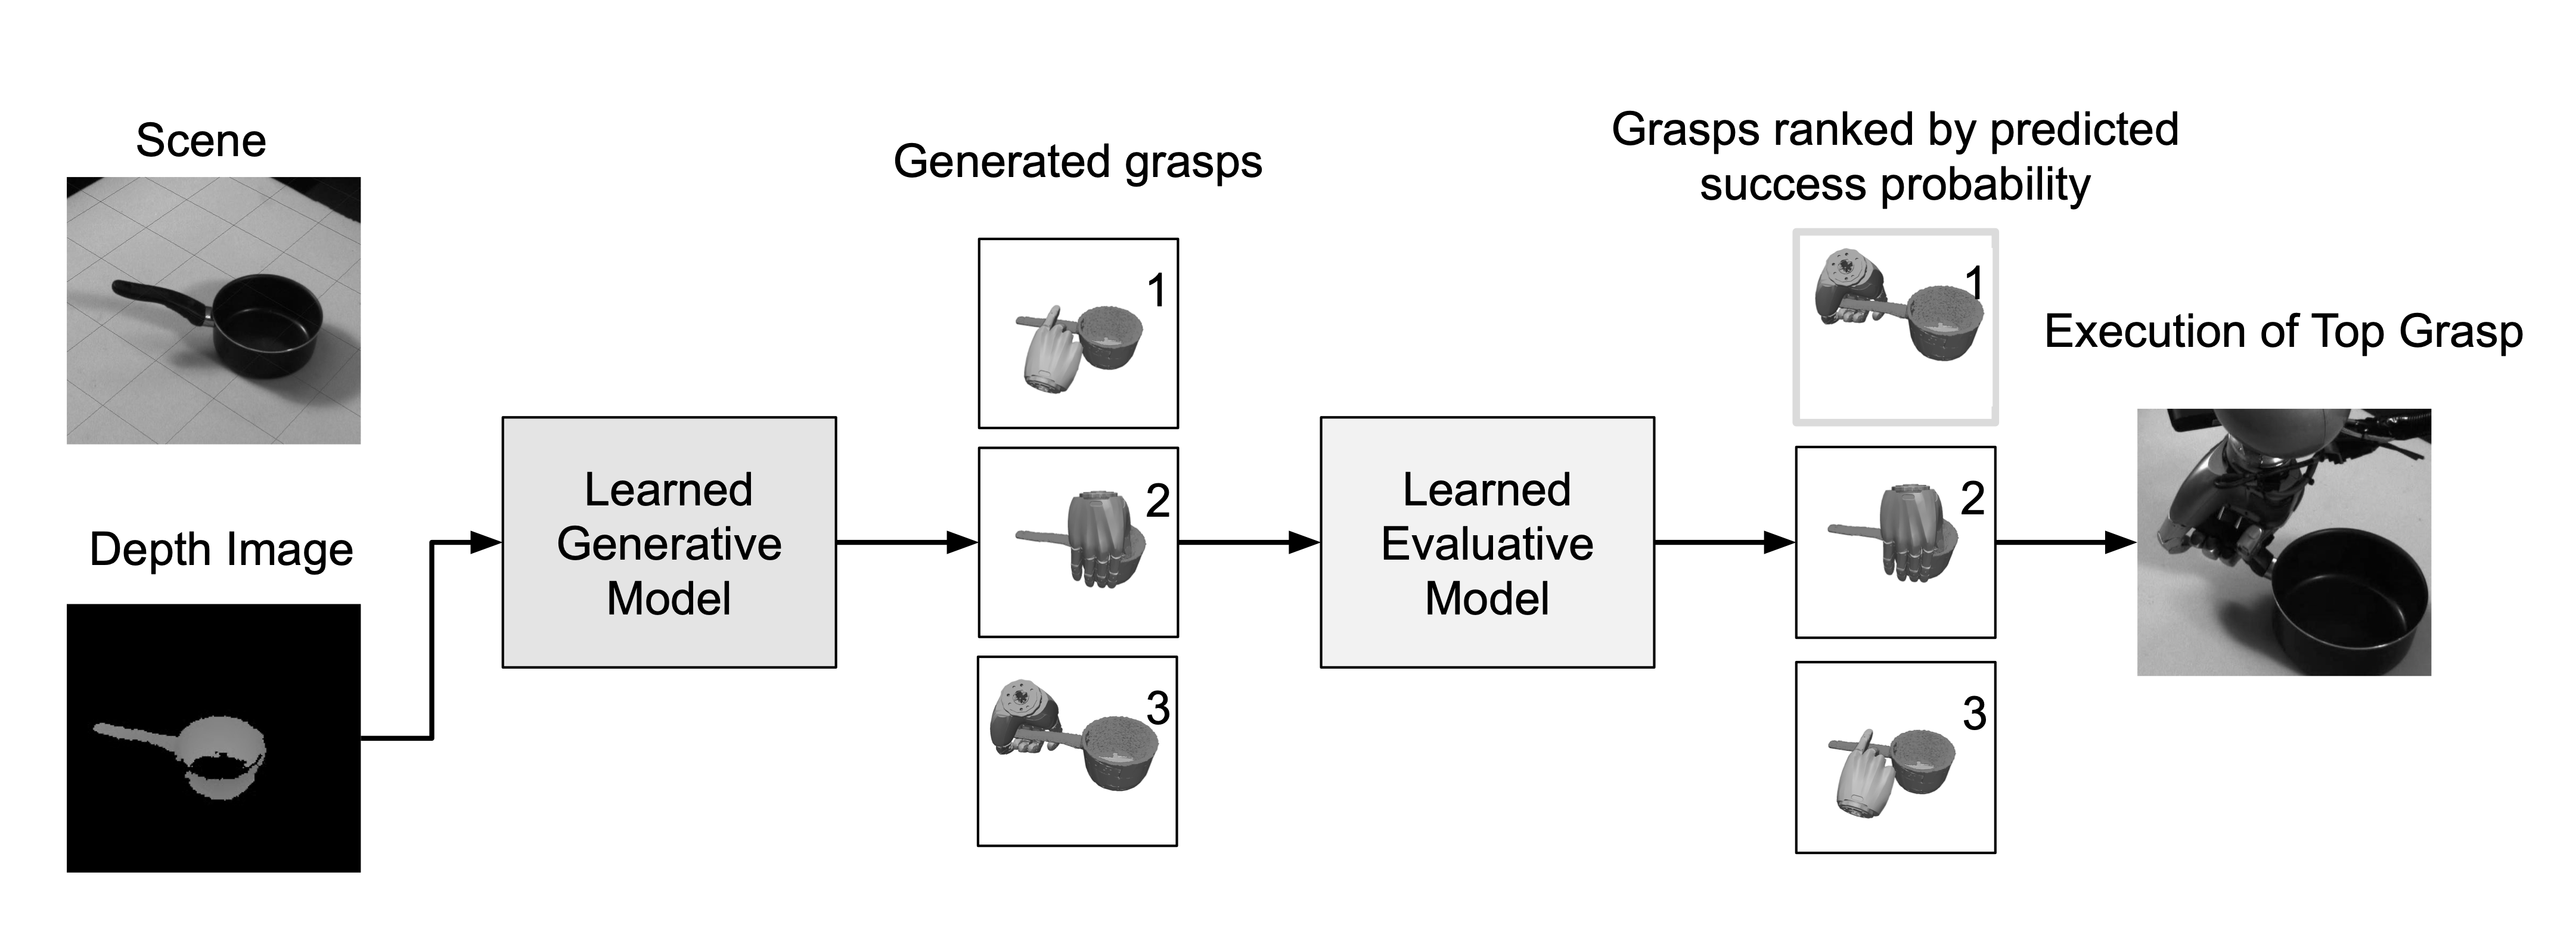
\includegraphics[width=\columnwidth]{images/GEAarchitecture.png}
  \end{center}
  \caption{Our grasping architecture. When shown an object, a generative model (GM) produces grasps, ranked according to its likelihood model. These are re-ranked by the predicted success probability of the evaluative Model (EM). The top ranked grasp is executed. \label{fig:systemArchitecture}}
\end{figure}

The contributions of this paper are as follows. First, we present a data set of 2.4m simulated dexterous grasps, available to evaluate dexterous grasping algorithms. Second, we release the source code of the dexterous grasp simulator, which can be used to visualise the data set and gather new data.\footnote{The code and simulated grasp data set are available at \href{https://rusen.github.io/DDG}{https://rusen.github.io/DDG}.} Third, we combine an existing learned generative model with multiple learned evaluative models that are trained from simulated grasps proposed by the generative model. Fourth, we present an extensive evaluation of all these models on our simulated data set. Fifth, we compare the two most promising variants on a real robot with a data set of objects in challenging poses. Finally, we perform a deep dive into the simulation results.

The model variants are organised in three dimensions. First, we employ two different generative models (GM1 \cite{kopicki2015ijrr} and GM2 \cite{kopicki2019ijrr}), one of which (GM2) is designed specifically for single view grasping. Second, we use two different back-bones for the evaluative model, VGG-16 and ResNet-50. Third, we experiment with two optimisation techniques--gradient ascent (GA) and stochastic annealing (SA)--to search for better grasps using the evaluative model as an objective function.

%The first contribution of this paper is the first generative-evaluative architecture where both generative and evaluative models are learned. Second, three novel evaluative networks, based on existing VGG-16 and ResNet-50 architectures, were proposed. Finally, a grasp simulation dataset containing 2M+ grasps on 295 objects, along with the simulator code will be released to to the community. In order to simulate the wide range of physical variations that real world objects have, a data set is acquired by simulation of  grasps proposed by the generative models on novel objects. We vary the physical characteristics of the objects in each simulated scene (mass, friction) which the robot can not observe. This dataset was used to train three evaluative neural networks. The evaluative models were then used to rank grasps produced by the generative models (GM1 and GM2) in real robot experiments. 

%The paper builds upon two existing generative grasp models that are learned from a small number of demonstrated grasps using the data-efficient method for LfD. Unlike other approaches to deep grasping, which are restricted to power-grasps, the methods are able to perform a wide variety of grasps, including pinch, rim, power, and handle grasps, and to use additional fingers to provide bracing.

The paper is structured as follows. First, we discuss related work. Second, we describe the design of the grasp simulation, the generation of the data set. Third, the proposed generative evaluative architecture is described and the different architectures employed for the evaluative model are explained, including the optimisation variants of the evaluative model. Fourth, a simulation-based experimental study of the proposed methods is presented. Fifth, we present the real robot study. Finally, we extend the simulation analysis further by examining the inner workings of the best performing model. 
